\documentclass[10pt]{book}
\usepackage{graphicx}
\usepackage{subfig} % make it possible to include more than one captioned figure/table in a single float
\usepackage[utf8]{inputenc}
\usepackage{hyperref}
\usepackage[intlimits]{amsmath}
\usepackage{amssymb}
\usepackage{float}
\setlength{\oddsidemargin}{15.5pt} 
\setlength{\evensidemargin}{15.5pt}
\pretolerance=2000
\tolerance=3000
\renewcommand{\figurename}{Figura}
\renewcommand{\chaptername}{Cap\'{i}tulo}
\renewcommand{\contentsname}{\'{I}ndice}
\renewcommand{\tablename}{Tabla}
\renewcommand{\bibname}{Bibliograf\'{i}a}
\renewcommand{\appendixname}{Ap\'endices}


\usepackage{geometry}
 \geometry{
 a4paper,
 left=5mm,
 right=5mm,
 top=5mm,
 bottom=5mm,
 }

\begin{document}

\paragraph {1a)} 
\begin{figure}[H]
 \centering
 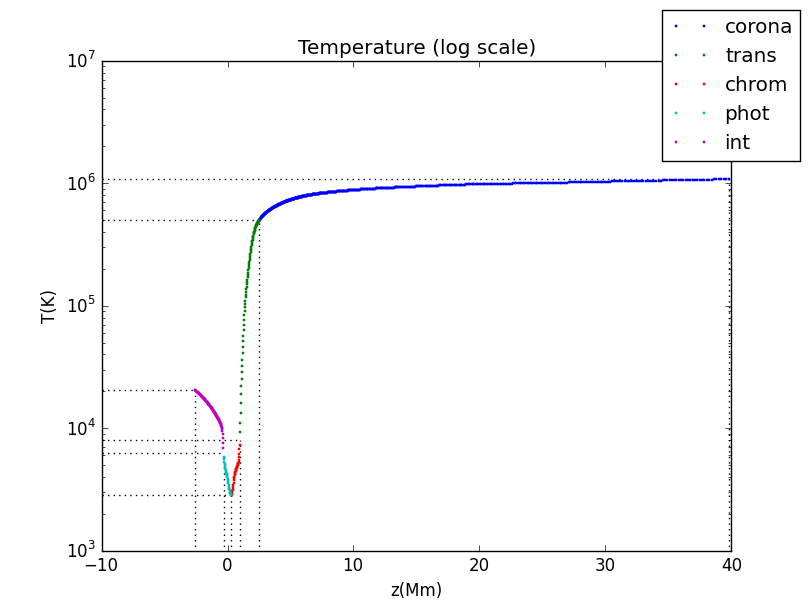
\includegraphics[scale=0.5]{tempLayers.png}
 \caption{\emph{Temperature vs z plot. logarithmic y scale}}
\end{figure}

In order to identify the layers I put conditions on temperature:

\url{http://www.nasa.gov/mission_pages/iris/multimedia/layerzoo.html}

Algorithm for getting the layers:
start with values at the top (the values from the  file 'atmosphere.dat' are ordered downwards by height) 
the corona is while temperature $\ge 500000$ K (T is decreasing), 
transition region until T = 8000 K, the chromosphere until T reaches the (only) minimum, (afterwards the temperature starts to raise) the photosphere  is before T reaches 6500 K and  the solar interior afetrwards until the end

The exact values matching these conditions are: 
\begin{description}

\item corona between [39.802200, 2.535930] Mm temperatures: [1.080180e+06, 5.025160e+05] K 
\item transition region between [2.516350, 0.991115] Mm temperatures: [4.991350e+05, 8.067640e+03] K  
\item chromosphere between [0.971556, 0.305708] Mm temperatures: [7.306160e+03, 2.843670e+03] K 
\item photosphere between [0.286093, -0.303487] Mm temperatures: [2.848470e+03, 6.297540e+03] K 
\item solar interior between [-0.323184, -2.592960] Mm temperatures: [6.837750e+03, 2.068340e+04] K 

\end{description}



\paragraph {1b)}

$\mu = \frac{n_{H} + 4 n_{He}}{n_e + n_H + n_{He}} $

$n_H= 10 n_{He} \implies  \mu = \frac{1.4 n_H}{n_e + 1.1 n_H}$


\begin{itemize}
\item totally ionized H and He $\implies n_e = n_H + 2 n_{He} = 1.2 n_H \implies \frac{n_H}{n_e} = \frac{5}{6} $ and 
$ \mu = 0.6087 $
\item neutral H and He $\implies n_e = 0 \implies  \mu = 1.2727 $

\end{itemize}



\begin{figure}[H]
 \centering
 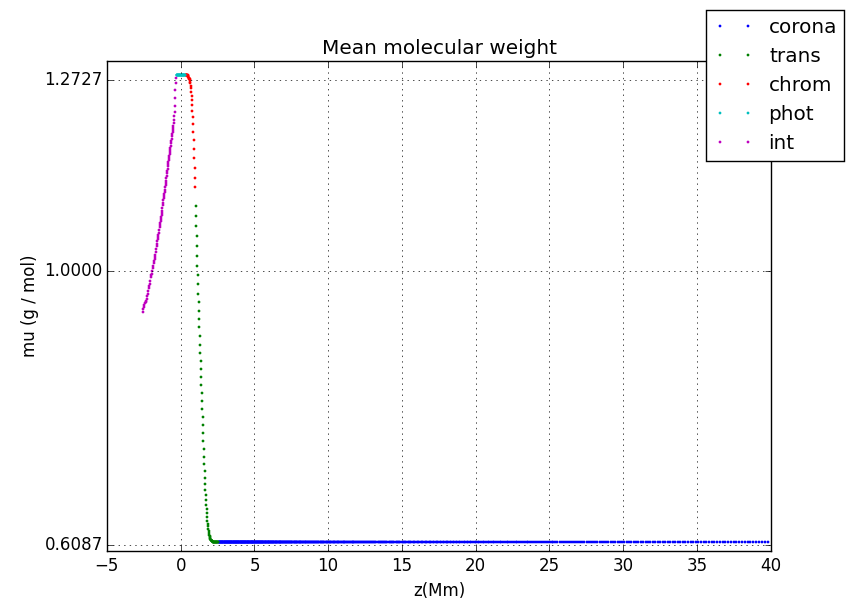
\includegraphics[scale=0.5]{mmmLayers.png}
 \caption{\emph{Mean molecular weight(g/mol) vs z plot} Maximum close to 1.2727 = $\mu$ in the case of neutral H and He and minimum close to 0.6087 = $\mu$ calculated in the case of completely ionized H and He }
\end{figure}

$\frac{n_H}{n_e} =  \frac{\mu}{1.4 - 1.1 \mu }   $

In the case of neutral H and He $n_e \rightarrow 0 \implies \frac{n_H}{n_e} \rightarrow \infty $

We expect to have big values of this variable in the photosphere

and as we can see in the graphic of $\mu$ there are some values of z for which

$\mu > 1.2727 \implies 1.4 - 1.1 \mu < 0 \implies \frac{n_H}{n_e} < 0$

I will limit oy axis values to $ [0,4]$ in order to avoid these negative values and the big ones 


\begin{figure}[H]
 \centering
 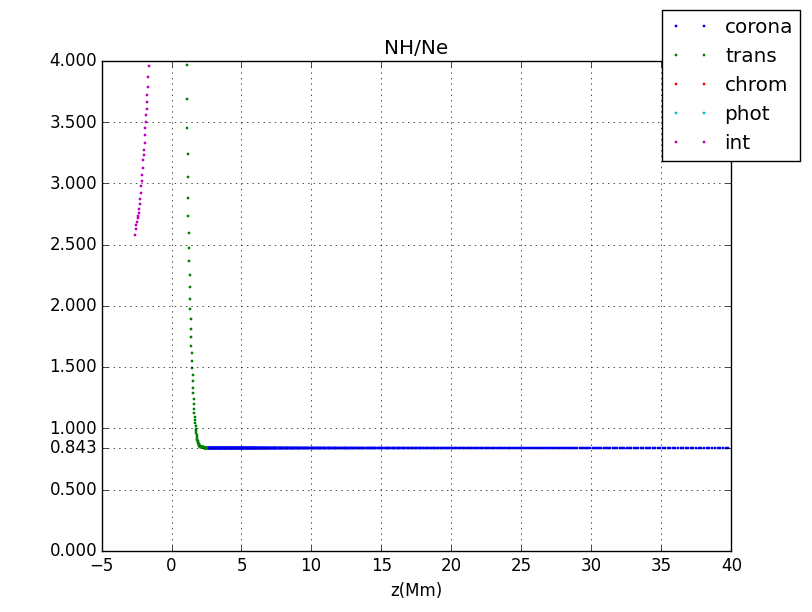
\includegraphics[scale=0.5]{nHDivNe.png}
 \caption{nH / ne }
\end{figure}

We can see a constant value  $\frac{n_H}{n_e}  = 0.843 \approx  \frac{5}{6}$ 
which is the value we calculate in the case of totally ionized H and He (we expect to have totally ionized H and He because of 
the high values of the temperature in the corona)



\begin{figure}[H]
 \centering
 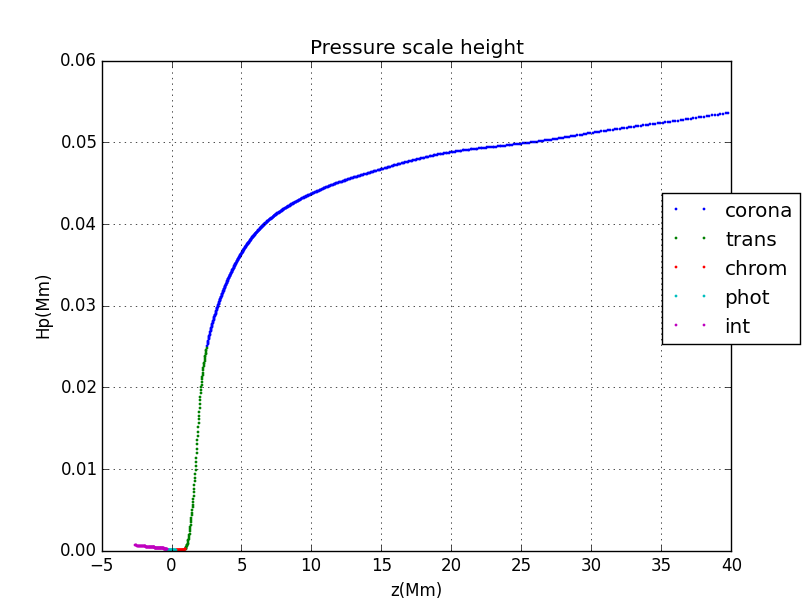
\includegraphics[scale=0.5]{hpLayers.png}
 \caption{Pressure scale height}
\end{figure}

\begin{figure}[H]
 \centering
 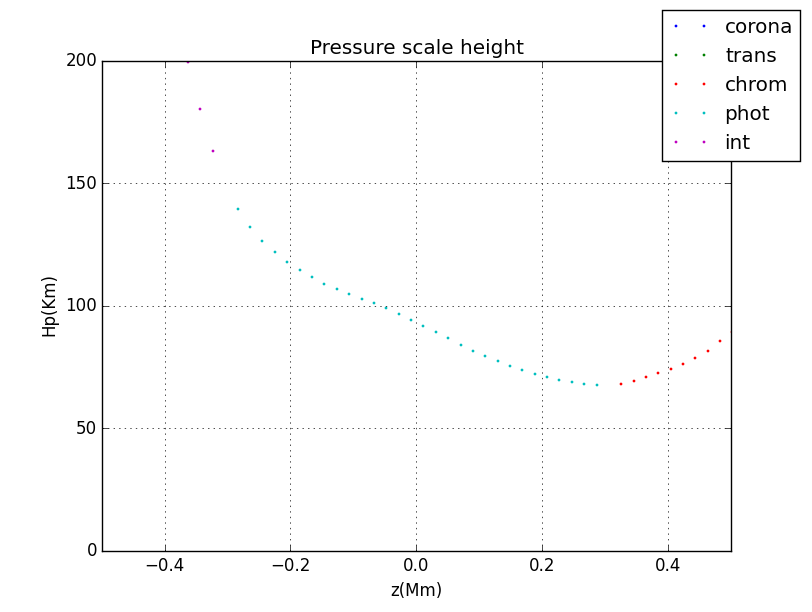
\includegraphics[scale=0.5]{hpLayersPart.png}
 \caption{Checking Hp in the photosphere (between approx 90 - 200 km)}
\end{figure}

Hp has the minimum at the bottom of the chromosphere (is where T has the minimum and $\mu$ the maximum and  $H_p \propto \frac{T}{\mu}$)

$H_p > 0 \implies $ pressure is a decreasing function. $H_p$ is the distance in which pressure will decrease by a factor e 
so a small value  like in the photosphere and chromosphere means that pressure will decrease fast in this portion




\paragraph{2)}

$\frac{d \text{ln} p}{dz} = -\frac{1}{H_p}$, $H_p$ const $\implies$ ln $p(z)$ - ln $ p(z_0) = -\frac{1}{H_p}(z-z_0) \implies p(z) = p(z_0) exp(-\frac{z-z_0}{H_p})$  

$\rho(z) =  \frac{1}{g H_p}p(z) = \frac{p(z_0)}{g H_p} exp(-\frac{z-z_0}{H_p}) = \rho(z_0) exp(-\frac{z-z_0}{H_p})$ 

Analytic test for $H_p$ constant (with values 1 and $1e10$) with $\rho(z_f)$ taking values: $1e-10, 1e-5, 1e-2,1, 1e2,1e3, 1e7, 1e10$
Integrating downward or forward in height makes no difference (using ln p)

We see that analytic solution matches exactly numerical solution(we plot ln $p(z)$ - ln $ p(z_i)$ vs z) and 

that the graphic is a line with slope $\frac{ln p(z_f) - ln  p(z_i)}{z_f - z_i} = -\frac{1}{H_p} $

where $z_f$ = $z_{max}$(z at the top of the atmosphere) and $z_i$ = $z_{min}$(z at the bottom of the atmosphere)


\begin{figure}[H]
 \centering
 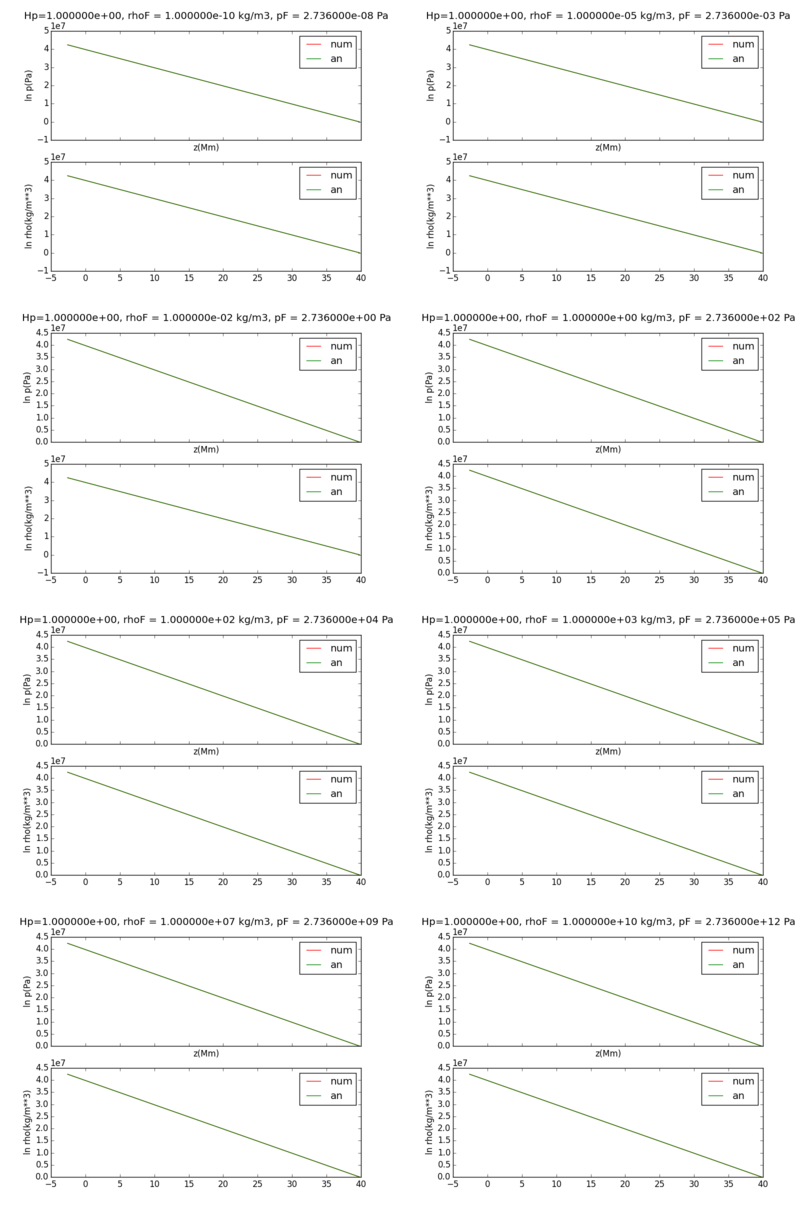
\includegraphics[scale=0.5]{allanalytic.png}
 \caption{Analytic test Hp=1e10}
\end{figure}


\begin{figure}[H]
 \centering
 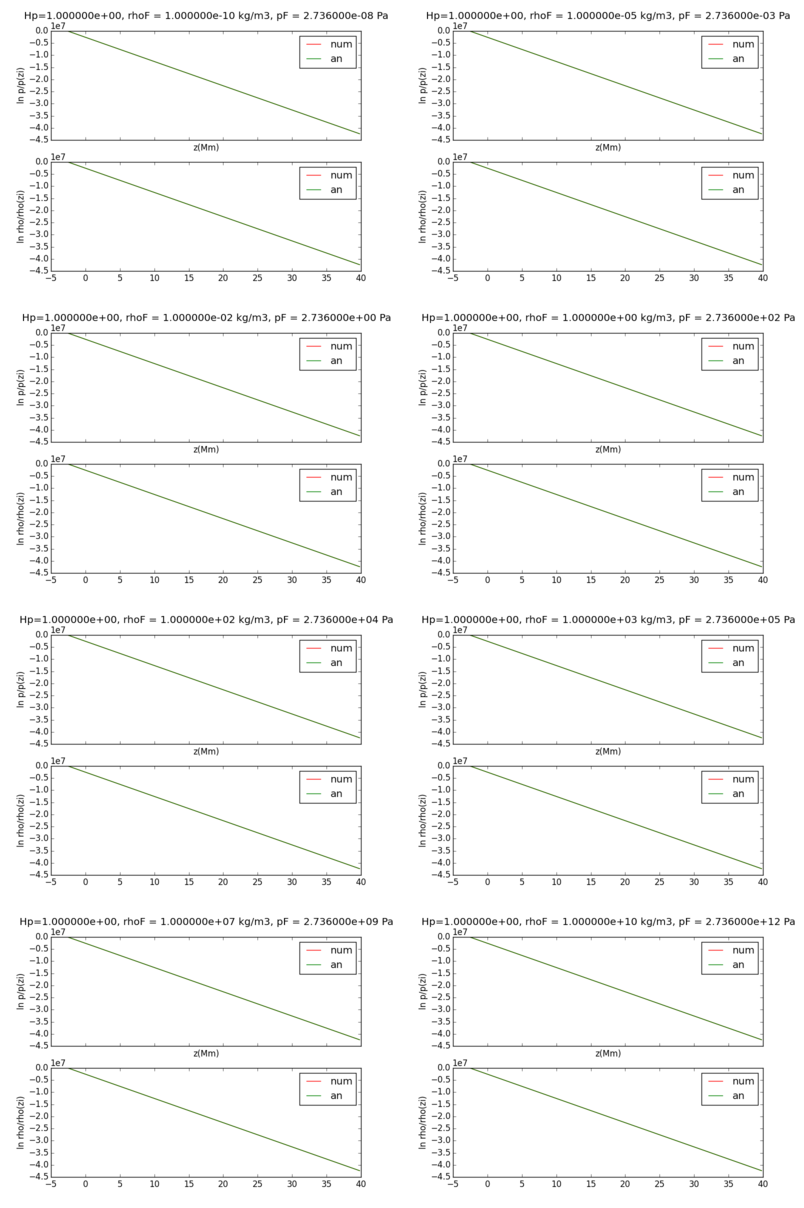
\includegraphics[scale=0.5]{allanalytic2.png}
 \caption{Analytic test Hp=1}
\end{figure}


\begin{figure}[H]
 \centering
 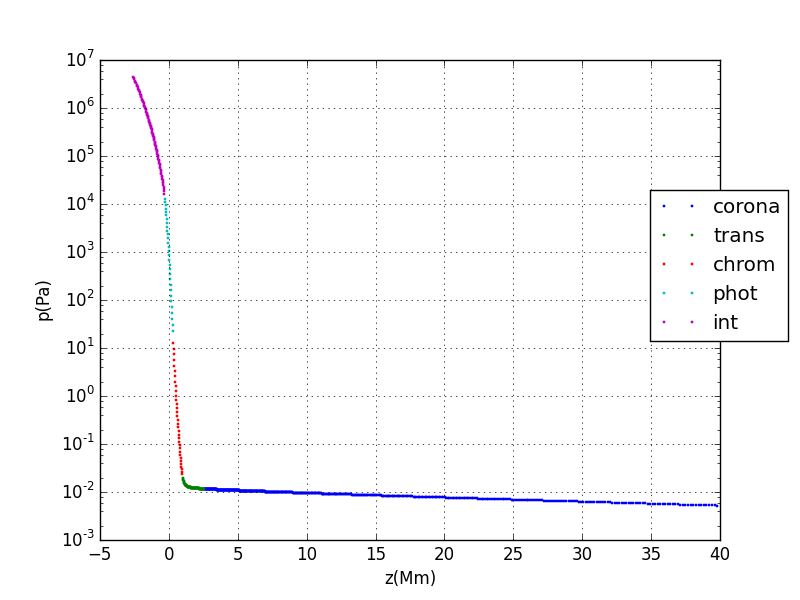
\includegraphics[scale=0.5]{fromFileLogScale1.png}
 \caption{pres log10 oy scale}
\end{figure}

\begin{figure}[H]
 \centering
 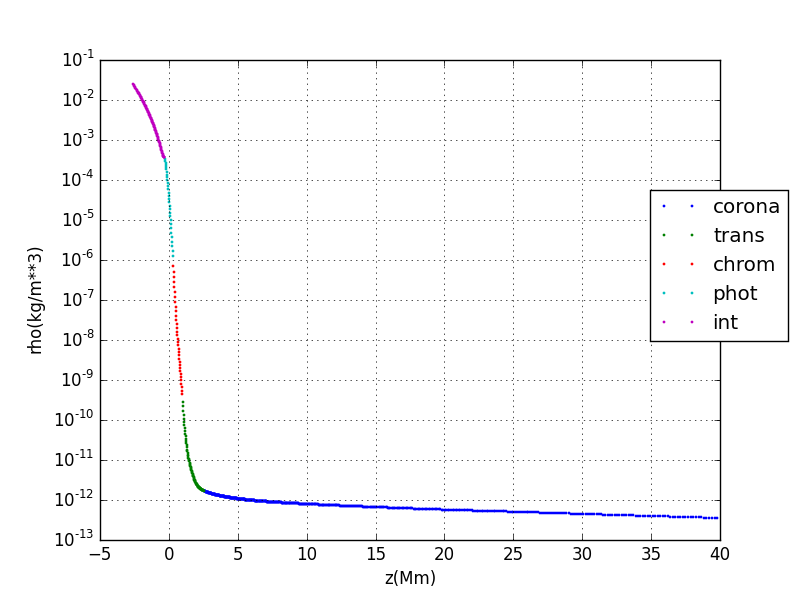
\includegraphics[scale=0.5]{fromFileLogScale2.png}
 \caption{rho log10 oy scale}
\end{figure}

Pressure will decrease very fast (a few orders of magnitude in a short distance) in the photosphere and chromosphere($H_p$ is very small in this portion )

In the transition zone and corona  pressure will decrease slowly because $H_p$ has now bigger values 

Density ($ \rho \propto \frac{p \mu}{T}$) will decrease fast in the transition zone as well because temperature raises very fast in this portion 

\paragraph{2b)}
Notation: $\mu_0$ = magnetic permeability 

$\beta = \frac{p}{p_{mag}}$ where $p_{mag} = \frac{B^2}{2 \mu_0}$

$v_A^2 = \frac{B ^2 }{ \mu_0 \rho} $

$c_s = \sqrt{\frac{\gamma p}{ \rho}} $

\begin{figure}[H]
 \centering
 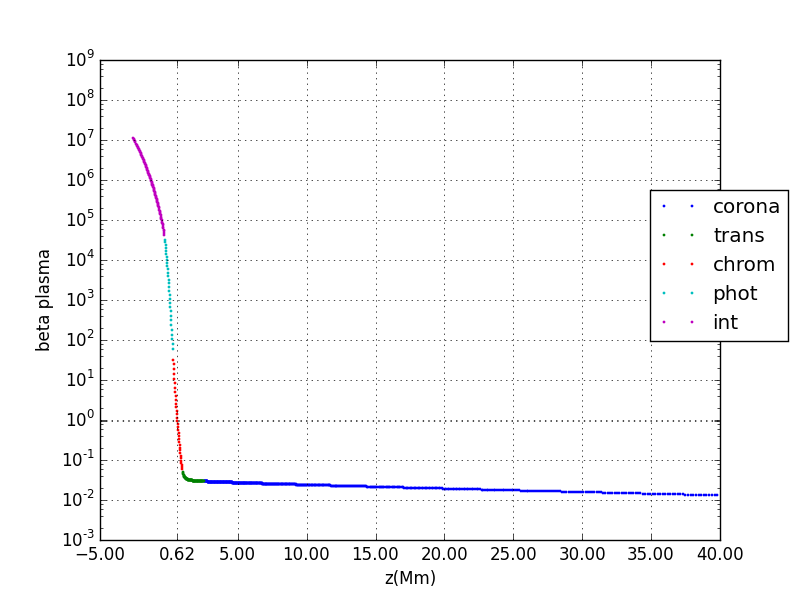
\includegraphics[scale=0.5]{fromFileLogScale3.png}
 \caption{plasma beta log10 oy scale}
\end{figure}

Plasma beta is a decreasing function and has value 1 at z = 0.62 Mm (in the chromosphere) 

\begin{figure}[H]
 \centering
 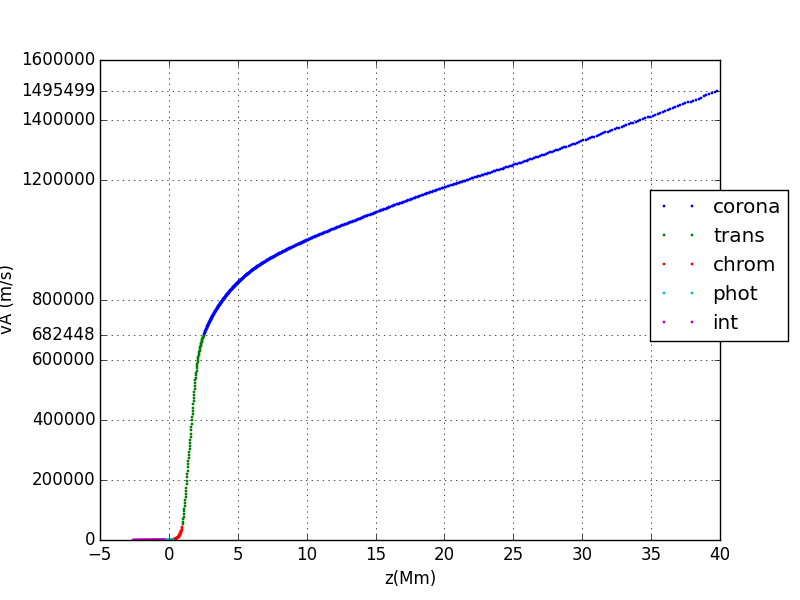
\includegraphics[scale=0.5]{fromFile4.png}
 \caption{vA}
\end{figure}

In the corona  we observe big values of vA  (between approx. 700 - 1500 km /s) ($vA \propto \rho^{-0.5}$) 

\begin{figure}[H]
 \centering
 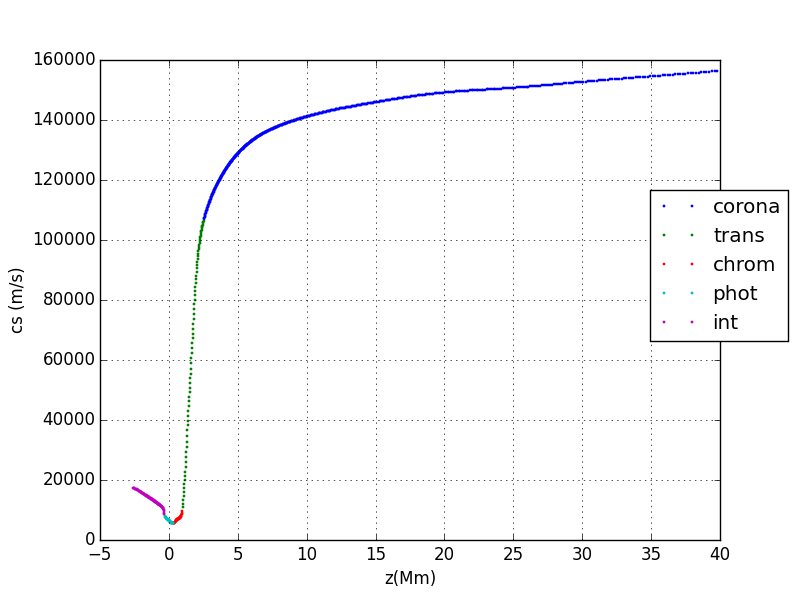
\includegraphics[scale=0.5]{fromFile5.png}
 \caption{cs}
\end{figure}

\begin{figure}[H]
 \centering
 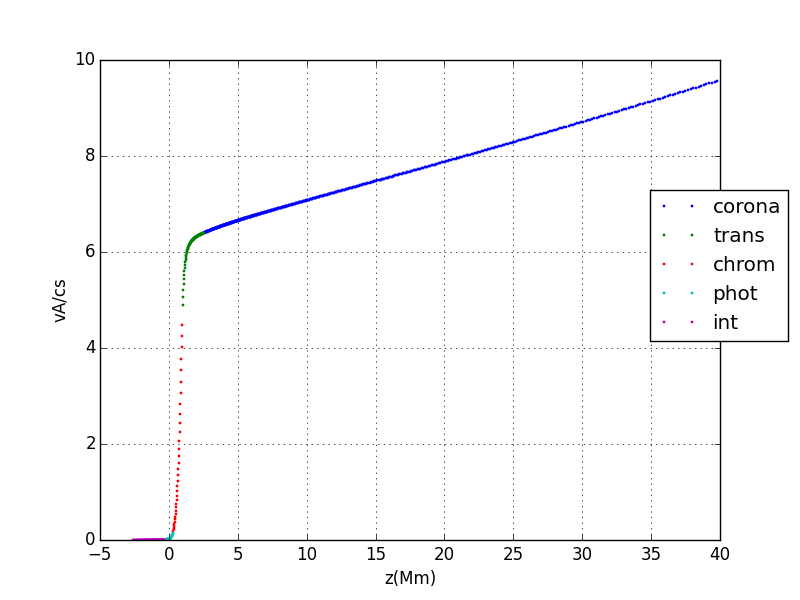
\includegraphics[scale=0.5]{fromFile6.png}
 \caption{vA/cs}
\end{figure}

In the corona $v_A > c_s$



$\beta = \frac{2 p \mu_0}{B^2} = \frac{2 p}{\rho v_A^2} = \frac{2 }{\gamma}(\frac{c_s}{v_A})^2
\implies \beta (\frac{v_A}{c_s})^2 \frac{\gamma}{2} = 1 $
We call this function func($\beta, \frac{v_A}{c_s}$) in the graphic below and expect it to be 1



\begin{figure}[H]
 \centering
 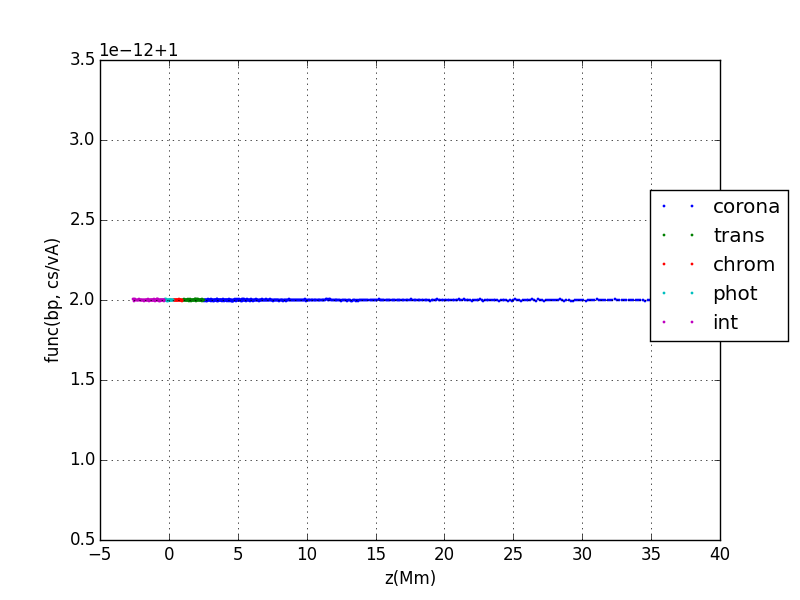
\includegraphics[scale=0.5]{fromFile7.png}
 \caption{func(bp, vA/cs) $\approx$ 1}
\end{figure}




\paragraph{3a)}

$L_r = \Lambda n_e n_H \implies $

in cgs:  $\frac{erg}{cm^3 s} = [\Lambda] \frac{1}{cm^6}$

units of $\Lambda$ in c.g.s are $\frac{erg cm^3}{s}$ 

\begin{figure}[H]
 \centering
 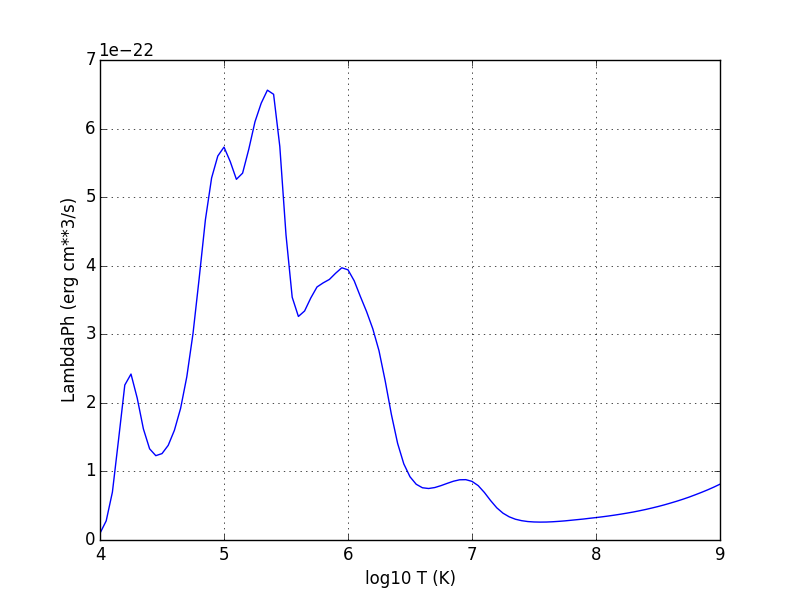
\includegraphics[scale=0.5]{lambdaPh.png}
 \caption{ Lambda phot}
\end{figure}

\begin{figure}[H]
 \centering
 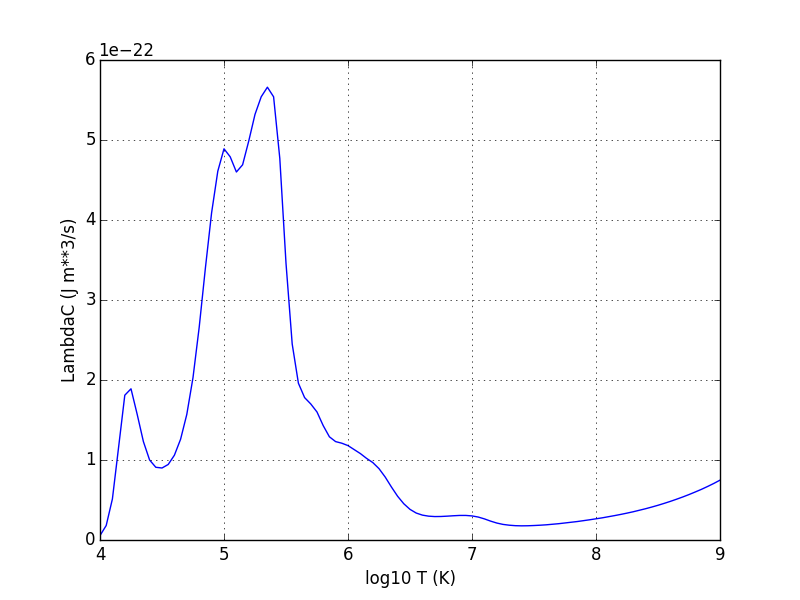
\includegraphics[scale=0.5]{lambdaC.png}
 \caption{ Lambda corona}
\end{figure}

Both functions have the maximum for T = 2.238721e+05 K

\paragraph{3b)}

$\rho = \sum_i n_i a_i m_H = (n_H + 4 n_{He}) m_H $

$n_H = 10 n_{He} \implies \rho = 1.4 n_H m_H$

\begin{figure}[H]
 \centering
 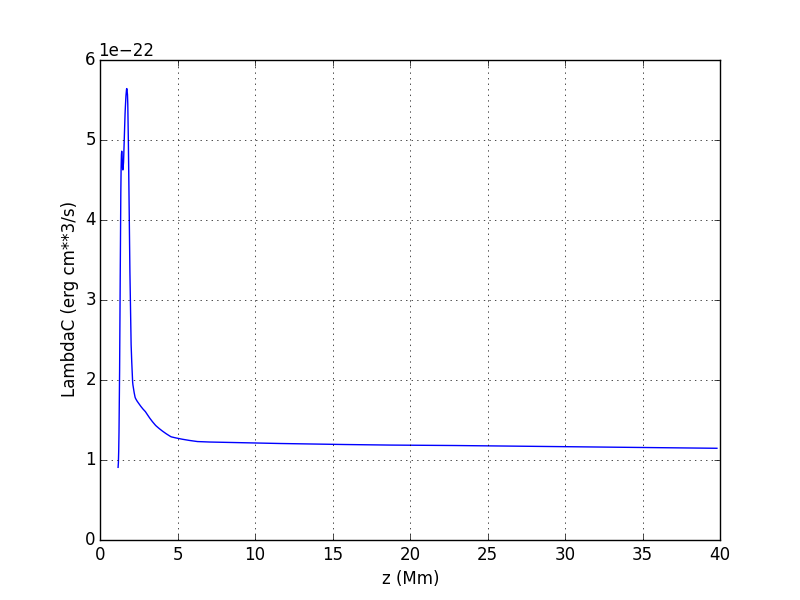
\includegraphics[scale=0.5]{interpLambdaC.png}
 \caption{ Lambda corona interpolated for atm. temperatures $> 3 * 10^4$ K in 'atmosphere.dat' plotted vs z}
\end{figure}

\begin{figure}[H]
 \centering
 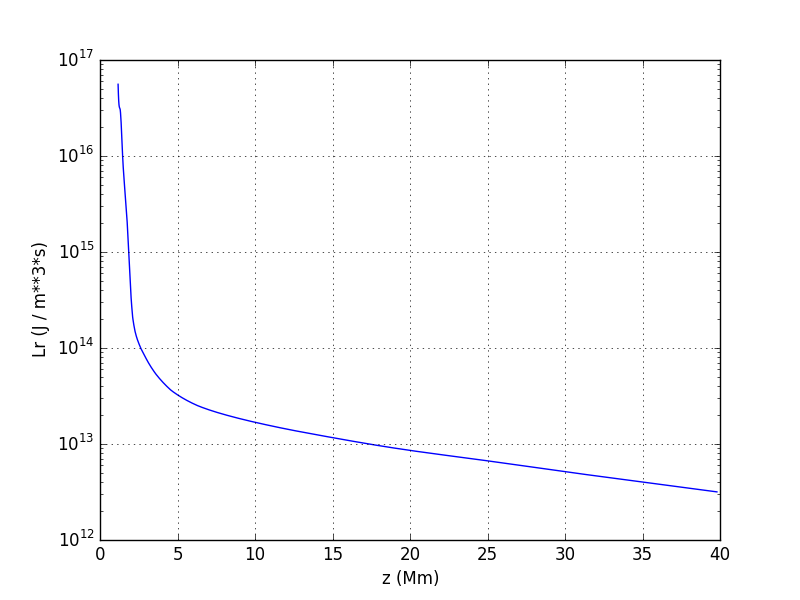
\includegraphics[scale=0.5]{Lr.png}
 \caption{ Lr}
\end{figure}


\paragraph{3c)}

\begin{figure}[H]
 \centering
 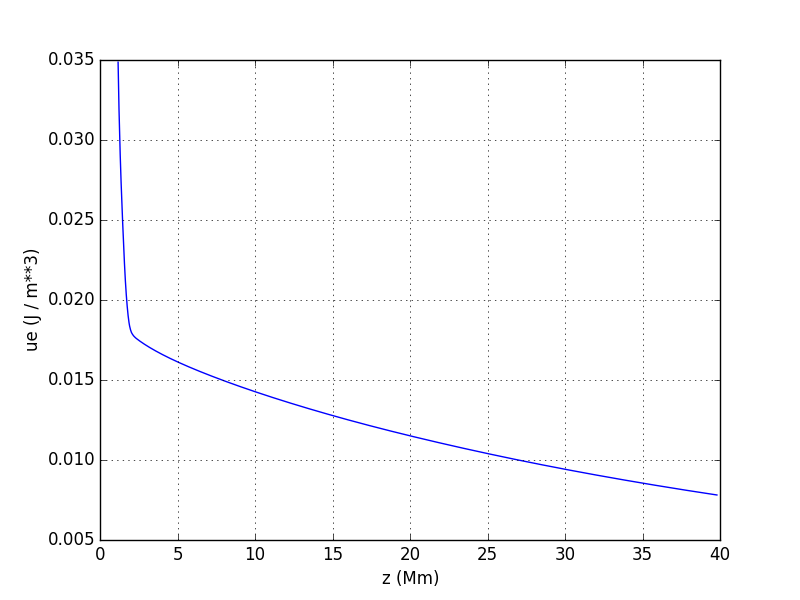
\includegraphics[scale=0.5]{ue.png}
 \caption{ Internal energy calculated as 1.5 * p}
\end{figure}

\paragraph{3d)}
Equation of energy when $\vec{q} = 0, \vec{v} = 0, \vec{j} = 0$:

$ \frac{\partial u_e}{\partial t} = -L_r$

if we consider $L_r$ constant in time(in fact $L_r$ will be decreasing in time because of its dependence on $n_e$ and T):

$u_e(t) = u_e(t=0) - L_r t \implies \frac{u_e(t=0)}{L_r}$ is the (minimum, if we think that
$L_r$ will decrease in time) time needed to convert all internal energy into radiation energy

units of $\frac{u_e(t=0)}{L_r}$ are units of time: s

\begin{figure}[H]
 \centering
 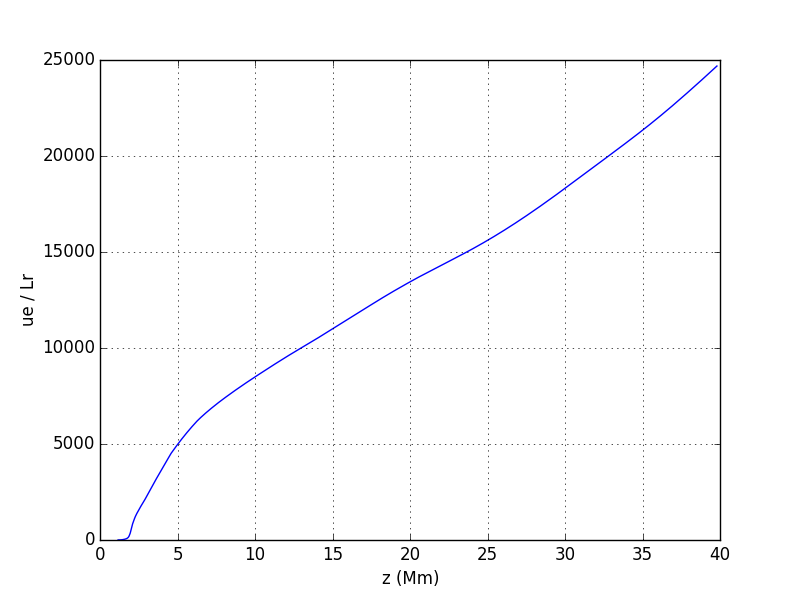
\includegraphics[scale=0.5]{ueDivLr.png}
 \caption{ Internal energy / Lr}
\end{figure}

The maximum value of $\frac{u_e(t=0)}{L_r} $ is about 25000 s at the top the corona, it needs more than  7 hours to cool completely

\paragraph{Testing}

Derivate ln p (obtained after integrating -1/Hp calculated with data taken from the file) by the following scheme:

for an array of n elements f[i], i in [0..n-1]
we calculate
df[i] = (f[i+1] - f[i-1]) / (dz[i-1] + dz[i]), for i in [1..n-2];
df[0] = df[1];
df[n-1] = df[n-2]

using dz[i] = z[i+1] - z[i] for i in [0..n-2]  (z taken from the file, we have both z and ln p reversed)

and for the array  d ln p obtained this way plot -1 / d ln p and compare with Hp

\begin{figure}[H]
 \centering
 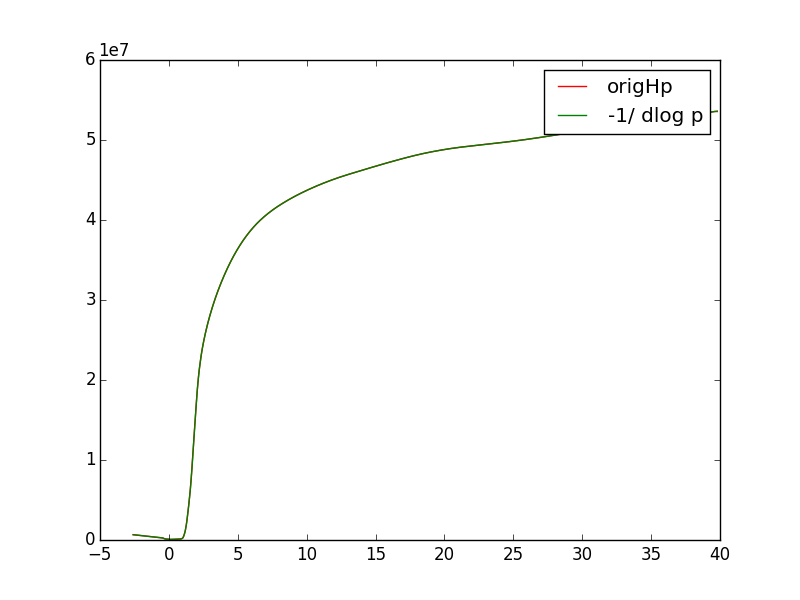
\includegraphics[scale=0.5]{fromFilePyTest.png}
 \caption{-1/d ln p = Hp}
\end{figure}


\paragraph{Resolution}

decrease resolution by taking off points: in one step we keep only points with even index in the array (first index is 0)

increase resolution artificially  by introducing points : in one step we add points in the middle between each 2 consecutive points and calculate
the functions from the table: $\mu$ and T by lineal or cubic interpolation


\begin{figure}[H]
 \centering
 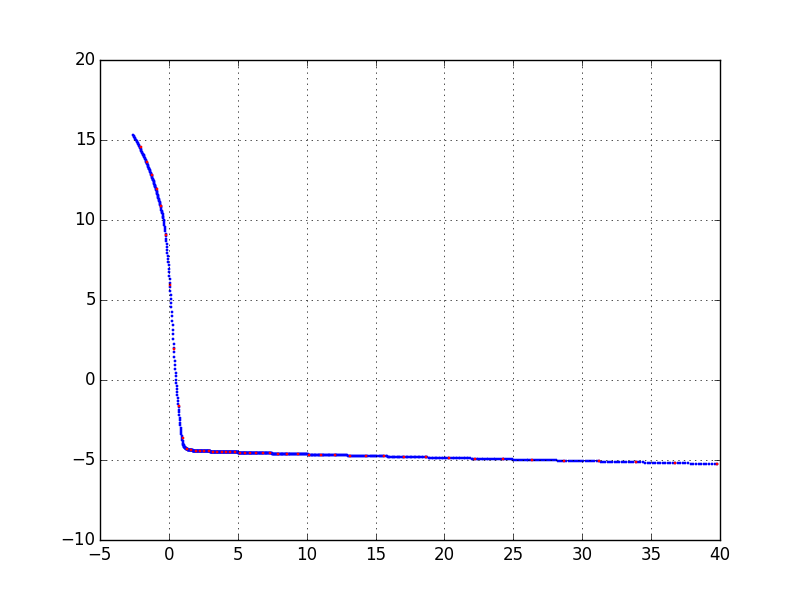
\includegraphics[scale=0.5]{testData48.png}
 \caption{ln p decreased resolution (4 steps): 48 points with red points plotted on top, original resolution 768 points }
\end{figure}

\begin{figure}[H]
 \centering
 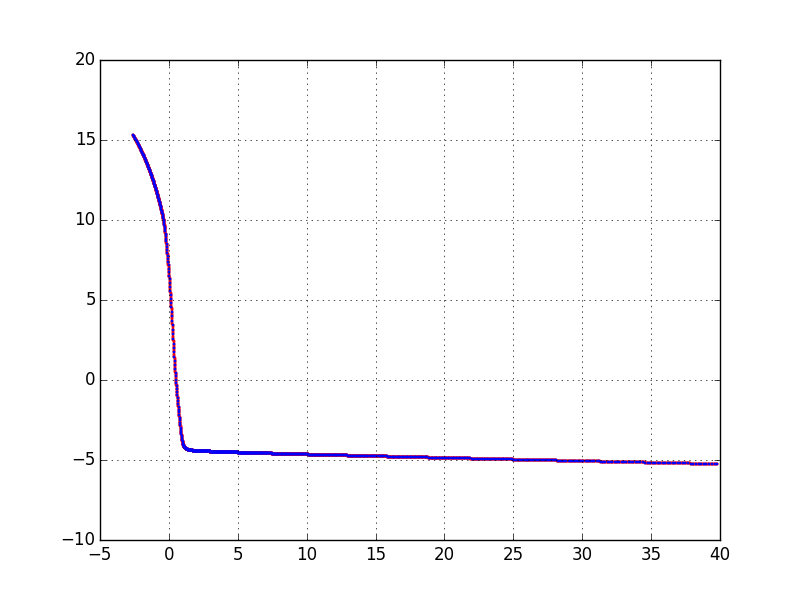
\includegraphics[scale=0.5]{testData3069.png}
 \caption{ln p increased resolution (2 steps, cubic interpolation): 3069 points with red points, original resolution 768 points plotted on top}
\end{figure}

\end{document}
